% This is a Basic Assignment Paper but with like Code and stuff allowed in it, there is also url, hyperlinks from contents included. 

\documentclass[11pt]{article}

% Preamble

\usepackage[margin=1in]{geometry}
\usepackage{amsfonts, amsmath, amssymb}
\usepackage{fancyhdr, float, graphicx}
\usepackage[utf8]{inputenc} % Required for inputting international characters
\usepackage[T1]{fontenc} % Output font encoding for international characters
\usepackage{fouriernc} % Use the New Century Schoolbook font
\usepackage[nottoc, notlot, notlof]{tocbibind}
\usepackage{listings}
\usepackage{xcolor}
\usepackage{blindtext}
\usepackage{hyperref}
\hypersetup{
    colorlinks=true,
    linkcolor=black,
    filecolor=magenta,      
    urlcolor=cyan,
    pdfpagemode=FullScreen,
    }

\definecolor{codegreen}{rgb}{0,0.6,0}
\definecolor{codegray}{rgb}{0.5,0.5,0.5}
\definecolor{codepurple}{rgb}{0.58,0,0.82}
\definecolor{backcolour}{rgb}{0.95,0.95,0.92}

\lstdefinestyle{mystyle}{
    backgroundcolor=\color{backcolour},   
    commentstyle=\color{codegreen},
    keywordstyle=\color{magenta},
    numberstyle=\tiny\color{codegray},
    stringstyle=\color{codepurple},
    basicstyle=\ttfamily\footnotesize,
    breakatwhitespace=false,         
    breaklines=true,                 
    captionpos=b,                    
    keepspaces=true,                 
    numbers=left,                    
    numbersep=5pt,                  
    showspaces=false,                
    showstringspaces=false,
    showtabs=false,                  
    tabsize=2
}

\lstset{style=mystyle}

% Header and Footer
\pagestyle{fancy}
\fancyhead{}
\fancyfoot{}
\fancyhead[L]{\textit{\Large{Internet of Things Lab Assignment 5}}}
\fancyhead[R]{\textit{\Large{Krishnaraj}}}
%\fancyhead[R]{\textit{something}}
\fancyfoot[C]{\thepage}
\renewcommand{\footrulewidth}{1pt}



% Other Doc Editing
% \parindent 0ex
%\renewcommand{\baselinestretch}{1.5}

\begin{document}

\begin{titlepage}
	\centering

	%---------------------------NAMES-------------------------------

	\huge\textsc{
		MIT World Peace University
	}\\

	\vspace{0.75\baselineskip} % space after Uni Name

	\LARGE{
		Internet of Things\\
		Second Year B. Tech, Semester 2
	}

	\vfill % space after Sub Name

	%--------------------------TITLE-------------------------------

	\rule{\textwidth}{1.6pt}\vspace*{-\baselineskip}\vspace*{2pt}
	\rule{\textwidth}{0.6pt}
	\vspace{0.75\baselineskip} % Whitespace above the title



	\huge{\textsc{
			Obstacle Detection and Notification using Arduino
		}} \\



	\vspace{0.5\baselineskip} % Whitespace below the title
	\rule{\textwidth}{0.6pt}\vspace*{-\baselineskip}\vspace*{2.8pt}
	\rule{\textwidth}{1.6pt}

	\vspace{1\baselineskip} % Whitespace after the title block

	%--------------------------SUBTITLE --------------------------	

	\LARGE\textsc{
		Assignment 5
	} % Subtitle or further description
	\vfill

	%--------------------------AUTHOR-------------------------------

	Prepared By
	\vspace{0.5\baselineskip} % Whitespace before the editors

	\Large{
		Krishnaraj Thadesar \\
		Cyber Security and Forensics\\
		Batch A2, PA 20
	}


	\vspace{0.5\baselineskip} % Whitespace below the editor list
	\today

\end{titlepage}


\tableofcontents
\thispagestyle{empty}
\clearpage

\setcounter{page}{1}

\section{Aim}

To simulate an operation of obstacle detection and notifying it with a buzzer or
LED using Raspberry-Pi/Beagle bone black board/ Tinker CAD Arduino etc.

\section{Objectives}
\begin{enumerate}
	\item To develop an obstacle detection system using Arduino, ultrasound sensor,
	      buzzer, and LED and or DC Motor.
	\item To demonstrate when the ultrasonic sensor detects an obstacle at an distance(3cm)
	      the Arduino orders the buzzer to ring and the red LED to light up.
\end{enumerate}

\section{Equipments Used}

\begin{table}[H]
	\begin{tabular}{|l|l|}
		\hline
		\textbf{Equipment Name} & \textbf{Quantity} \\ \hline
		Raspberry Pi Model 3 B  & 1                 \\ \hline
		DC Motor                & 1                 \\ \hline
		Ultrasonic Sensor       & 1                 \\ \hline
	\end{tabular}
\end{table}

\section{Theory}
The objective of this project is to develop an obstacle detection system using an Arduino microcontroller, an ultrasonic sensor, a buzzer, and a LED or a DC motor. The ultrasonic sensor is used to detect obstacles within a certain range, and when an obstacle is detected, the Arduino will activate the buzzer and the LED or the DC motor. This system can be useful in various applications, such as in automobiles, robots, and security systems, where obstacle detection is important.\\

In this project, the ultrasonic sensor is used to measure the distance between the sensor and the obstacle. The sensor emits high-frequency sound waves and then listens for the echo of those waves bouncing back from the obstacle. The time between the transmission and reception of the sound waves is used to calculate the distance between the sensor and the obstacle.\\

The ultrasonic sensor used in this project is the HC-SR04, which has four pins: VCC, GND, Trigger, and Echo. The VCC and GND pins are connected to the 5V and GND pins of the Arduino, respectively. The Trigger pin is used to send the ultrasonic sound wave, and the Echo pin is used to receive the echo of the sound wave.\\

The LED or the DC motor is used to provide a visual or a physical indication of the obstacle detection. The LED is connected to a digital output pin of the Arduino, and it can be turned on or off by writing a high or low value to that pin. \\

The DC motor is connected to a motor driver module, which is connected to two digital output pins of the Arduino. By varying the voltage and the polarity of the output pins, the direction and the speed of the DC motor can be controlled.\\

In the context of the Internet of Things (IoT), this project can be extended to include wireless communication between the Arduino and other devices or systems. For example, the Arduino can be connected to a Wi-Fi or a Bluetooth module, which can be used to send the obstacle detection data to a cloud server or a smartphone application. The data can then be processed and analyzed to provide insights and actions based on the detected obstacles.\\

This can be useful in smart city applications, where the traffic flow can be optimized based on the real-time obstacle detection data. The use of wireless communication in IoT also enables remote monitoring and control of the obstacle detection system, making it more efficient and convenient.

\section{Circuit Diagram}
\begin{figure}[H]
	\centering
	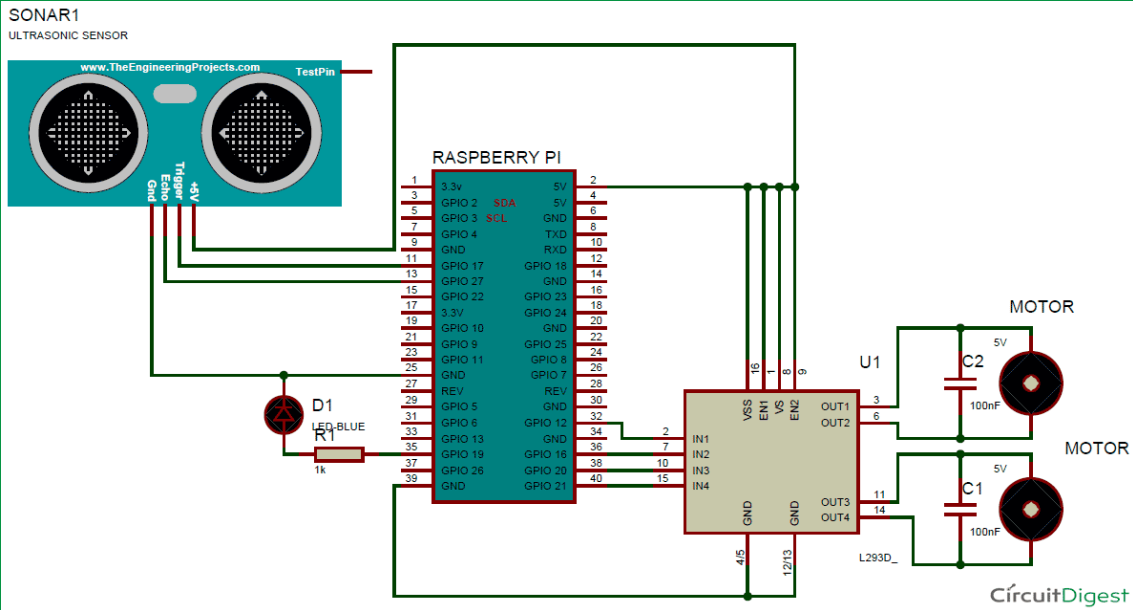
\includegraphics[width=.95\textwidth]{Screenshot_on_2023-05-01_at_22-55-37.png}
	\caption{Circuit Diagram}
\end{figure}

\section{Platform}
\textbf{Operating System}: Arch Linux x86-64 \\
\textbf{IDEs or Text Editors Used}: Visual Studio Code and Tinkercad, thonny on Pi\\
% \textbf{Compilers} : g++ and gcc on linux for C++, and javac, with JDK 18.0.2 for Java\\

\section{Input}
Data from the Ultrasonic sensor is given to pi.
\section{Output}
\begin{figure}[H]
	\centering
	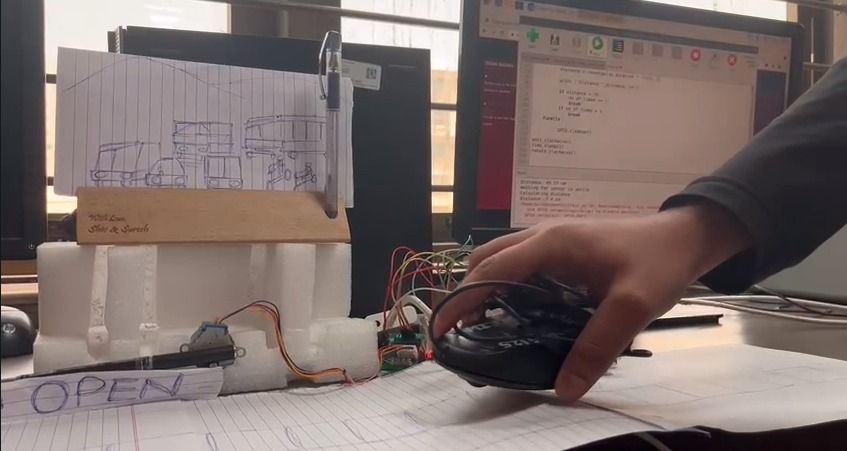
\includegraphics[width=.95\textwidth]{WhatsApp Image 2023-05-01 at 17.24.16.jpeg}
	\caption{Demonstration of the Project}
\end{figure}

\section{Code}
\begin{lstlisting}[language=python]
	import RPi.GPIO as GPIO
	import time
	GPIO.setmode(GPIO.BOARD)
	control_pins = [7,11,13,15]
	
	#Clockwise direction
	for pin in control_pins:
	  GPIO.setup(pin, GPIO.OUT)
	  GPIO.output(pin, 0)
	halfstep_seq = [
	  [1,0,0,0],
	  [1,1,0,0],
	  [0,1,0,0],
	  [0,1,1,0],
	  [0,0,1,0],
	  [0,0,1,1],
	  [0,0,0,1],
	  [1,0,0,1]
	]
	for i in range(512):
	  for halfstep in range(8):
		for pin in range(4):
		  GPIO.output(control_pins[pin], halfstep_seq[halfstep][pin])
		time.sleep(0.002)
	
	#Anti Clockwise direction
	for pin in control_pins:
	  GPIO.setup(pin, GPIO.OUT)
	  GPIO.output(pin, 0)
	halfstep_seq = [
	  [1,0,0,1],
	  [0,0,0,1],
	  [0,0,1,1],
	  [0,0,1,0],
	  [0,1,1,0],
	  [0,1,0,0],
	  [1,1,0,0],
	  [1,0,0,0]
	]
	for i in range(512):
	  for halfstep in range(8):
		for pin in range(4):
		  GPIO.output(control_pins[pin], halfstep_seq[halfstep][pin])
		time.sleep(0.002)
	GPIO.cleanup()

	print ("Script for Controlling Distance Sensor")

try:
      GPIO.setmode(GPIO.BOARD)
      PIN_TRIGGER = 7
      PIN_ECHO = 11
      GPIO.setup(PIN_TRIGGER, GPIO.OUT)
      GPIO.setup(PIN_ECHO, GPIO.IN)
      GPIO.output(PIN_TRIGGER, GPIO.LOW)
      print ("Waiting for sensor to settle")
      time.sleep(2)
      print ("Calculating distance")
      GPIO.output(PIN_TRIGGER, GPIO.HIGH)
      time.sleep(0.00001)
      GPIO.output(PIN_TRIGGER, GPIO.LOW)
      while GPIO.input(PIN_ECHO)==0:
            pulse_start_time = time.time()
      while GPIO.input(PIN_ECHO)==1:
            pulse_end_time = time.time()
      pulse_duration = pulse_end_time - pulse_start_time
      distance = round(pulse_duration * 17150, 2)
      print ("Distance:",distance,"cm")

finally:

      GPIO.cleanup()
\end{lstlisting}
\section{Conclusion}
Thus, we have successfully simulated an operation of obstacle detection and notifying it with a DC motor.
\clearpage

\section{FAQ}

Details of the main components used in this project and their pin specifications:

\begin{enumerate}
	\item Raspberry Pi Model 3 B: \\
	      The Raspberry Pi has a total of 40 pins, including 26 GPIO (General Purpose Input/Output) pins, 3.3V and 5V power pins, and ground pins. The pinout diagram for the Raspberry Pi 3 B can be found on the official Raspberry Pi website.

	      \begin{itemize}
		      \item Pin 1: 3.3V
		      \item Pin 2: 5V
		      \item Pin 3: GPIO 2
		      \item Pin 4: 5V
		      \item Pin 5: GPIO 3
		      \item Pin 6: Ground
		      \item Pin 7: GPIO 4
		      \item Pin 8: GPIO 14
		      \item Pin 9: Ground
		      \item Pin 10: GPIO 15
		      \item Pin 11: GPIO 17
		      \item Pin 12: GPIO 18
		      \item Pin 13: GPIO 27
		      \item Pin 14: Ground
		      \item Pin 15: GPIO 22
		      \item Pin 16: GPIO 23
		      \item Pin 17: 3.3V
		      \item Pin 18: GPIO 24
		      \item Pin 19: GPIO 10
		      \item Pin 20: Ground
		      \item Pin 21: GPIO 9
		      \item Pin 22: GPIO 25
		      \item Pin 23: GPIO 11
		      \item Pin 24: GPIO 8
		      \item Pin 25: Ground
		      \item Pin 26: GPIO 7
		      \item Pin 27: ID SD
		      \item Pin 28: ID SC
		      \item Pin 29: GPIO 5
		      \item Pin 30: Ground
		      \item Pin 31: GPIO 6
		      \item Pin 32: GPIO 12
		      \item Pin 33: GPIO 13
		      \item Pin 34: Ground
		      \item Pin 35: GPIO 19
		      \item Pin 36: GPIO 16
		      \item Pin 37: GPIO 26
		      \item Pin 38: GPIO 20
		      \item Pin 39: Ground
		      \item Pin 40: GPIO 21
	      \end{itemize}
	\item DC Motor: \\
	      A DC motor typically has two wires for power and two wires for control. The power wires are typically red and black, and the control wires can be any other color. The control wires are used to vary the voltage and polarity of the applied power to control the speed and direction of the motor.
	\item Ultrasonic Sensor (HC-SR04): The HC-SR04 ultrasonic sensor has four pins: Vcc, Trig, Echo, and Gnd. The pin specifications are as follows:
	      \begin{itemize}
		      \item Vcc: This pin is used to provide power to the sensor. It typically requires a voltage of 5V, but it can also be powered using 3.3V.
		      \item Trig: This pin is a digital output pin that is used to trigger the sensor. It sends a 10µs pulse to the sensor to start the measurement.
		      \item Echo: This pin is a digital input pin that receives the echo signal. It measures the time taken for the ultrasonic waves to travel to the object and back, and sends a pulse back to the Raspberry Pi to indicate the distance.
		      \item Gnd: This pin is used to connect the sensor to ground.
	      \end{itemize}
\end{enumerate}

\end{document}